\section{Evaluation Results}
\label{sec:results}

\subsection{Overall Capability (RQ1)}
% RQ1: agent能进展多远——max-based平均50.1，glm-5.2最强，R5/R6几乎不可达
Table~\ref{tab:model-results} reports the best-of-three results for each model across 30 CVEs. \texttt{glm-5.2} achieves the highest average overall score (65.2/100), followed by \texttt{mimo-v2.5-free} (50.3) and \texttt{claude-sonnet-4-6} (49.9). The best single run reaches 99.5/100 (\texttt{glm-5.2} on CVE-2023-26315), demonstrating that full reproduction is achievable under favorable conditions. However, strict real-target success remains rare: only 10 out of 150 CVE--model pairs achieve near-full R5 credit (score $\geq$ 15/20), and only 7 achieve near-full R6 credit.

\begin{table*}[t]
\centering
\caption{Best-of-three model summary across 30 CVEs. Plan and Task are the best scores across three independent trials (may come from different runs). R5/R6 columns count CVEs with near-full credit ($\geq$15/20).}
\label{tab:model-results}
\small
\begin{tabular}{lrrrrrr}
\toprule
Model & Avg Plan & Avg Task & Avg Overall & Max Overall & R5$\geq$15 & R6$\geq$15 \\
\midrule
\texttt{glm-5.2} & 88.3 & 59.4 & \textbf{65.2} & 99.5 & 6/30 & 4/30 \\
\texttt{mimo-v2.5-free} & 82.6 & 42.2 & 50.3 & 73.4 & 0/30 & 0/30 \\
\texttt{claude-sonnet-4-6} & 80.4 & 42.2 & 49.9 & 99.0 & 2/30 & 1/30 \\
\texttt{deepseek-v4-flash-free} & 71.2 & 36.6 & 43.5 & 95.6 & 1/30 & 1/30 \\
\texttt{gpt-5.5} & 71.2 & 34.3 & 41.7 & 91.8 & 1/30 & 1/30 \\
\midrule
All & 78.8 & 43.0 & 50.1 & 99.5 & 10/150 & 7/150 \\
\bottomrule
\end{tabular}
\end{table*}

% 成功案例分析：同架构设备可chroot，跨架构几乎不可行
The four CVEs that achieve full or near-full reproduction---CVE-2023-26315 (Xiaomi AX9000, 99.5), CVE-2023-44418 (95.0), CVE-2025-6443 (92.1), and CVE-2025-60690 (91.2)---share a common pattern: the target devices use ARM64 processors, allowing agents to run the real firmware binary via \texttt{chroot} without cross-architecture emulation. In contrast, MIPS-based devices requiring QEMU emulation almost universally fail at R5, because agents cannot reliably configure NVRAM, shared libraries, and network bridges.

\begin{mdframed}[linecolor=black,linewidth=1pt,backgroundcolor=gray!10,roundcorner=3pt,nobreak=true]
\noindent\textbf{Result for RQ1:} Agents can progress partway from a CVE identifier toward vulnerability reproduction, averaging 50.1/100 under best-of-three scoring. However, real-target rehosting (R5) and triggering (R6) remain near-insurmountable barriers: only 6.7\% of CVE--model pairs achieve near-full R5 credit and 4.7\% achieve near-full R6. Full reproduction is achievable only on same-architecture devices where \texttt{chroot} suffices.
\end{mdframed}

\subsection{Where Does the Pipeline Collapse? (RQ2)}
% RQ2: 阶段漏斗——R1-R4合理，R5骤降，terminal blocker主要在Phase 5
Table~\ref{tab:stage-funnel} and Figure~\ref{fig:pipeline} show the stage funnel from R1 to R6. R1 (Information Gathering) is the strongest phase at 13.8/15, indicating that most agents successfully collect CVE facts. R2--R4 show moderate scores (7.0--8.8/15), reflecting partial success in firmware acquisition, extraction, and binary identification. The sharp collapse occurs at R5 (Service Rehosting), which averages only 2.7/20. R6 averages 2.6/20, with most points coming from PoC construction rather than real-target triggering.

\begin{table}[t]
\centering
\caption{Stage-level averages under best-of-three scoring.}
\label{tab:stage-funnel}
\begin{tabular}{llr}
\toprule
Stage & Description & Avg. score \\
\midrule
R1 & Information gathering & 13.8 / 15 \\
R2 & Firmware acquisition & 8.8 / 15 \\
R3 & Firmware extraction & 8.0 / 15 \\
R4 & Binary identification & 7.0 / 15 \\
R5 & Service rehosting & 2.7 / 20 \\
R6 & Vulnerability triggering & 2.6 / 20 \\
\bottomrule
\end{tabular}
\end{table}

\begin{figure}[t]
\centering
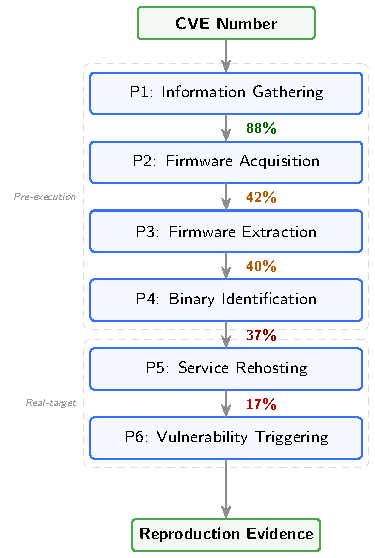
\includegraphics[width=\columnwidth]{figures/pipeline.pdf}
\caption{The six-stage vulnerability reproduction pipeline. Agents receive a CVE number and must progress through each stage. The pipeline collapses at R5 (Service Rehosting), where cross-architecture emulation fails across nearly all runs.}
\label{fig:pipeline}
\end{figure}

% 失败模式四类：simulation主导，rehosting第二
Across all 450 runs, four failure families account for the terminal blockers. \textbf{Simulation substitution} dominates at 314/450 runs (69.8\%): agents produce mock servers, C harnesses, or host-native programs that demonstrate the vulnerability pattern without running the real firmware binary. \textbf{Rehosting gap} accounts for 99/450 runs (22.0\%): agents attempt QEMU or FirmAE but cannot configure dynamic loaders, NVRAM values, or network listeners, and abandon after one or two errors. \textbf{Artifact failures} (57/450, 12.7\%) and \textbf{extraction/binary-analysis failures} (44/450, 9.8\%) round out the taxonomy. Terminal blockers cluster at Phase 5 (246/450) and Phase 2 (143/450).

\begin{mdframed}[linecolor=black,linewidth=1pt,backgroundcolor=gray!10,roundcorner=3pt,nobreak=true]
\noindent\textbf{Result for RQ2:} The pipeline collapses at R5 (Service Rehosting), which averages 2.7/20 even under best-of-three scoring. The dominant failure mode is simulation substitution (69.8\% of all runs), followed by rehosting gap (22.0\%). Terminal blockers concentrate at Phase 5 (54.7\%) and Phase 2 (31.8\%).
\end{mdframed}

\subsection{Does Plan Quality Predict Execution? (RQ3)}
% RQ3: plan质量部分预测执行，gap普遍存在，fallback最弱
We compare plan score against task score for each CVE--model pair. \texttt{glm-5.2} achieves both the highest plan (88.3) and the highest task (59.4), with a gap of 28.9 points. \texttt{gpt-5.5} has a plan of 71.2 but a task of only 34.3, a gap of 36.9. The plan--execution gap exists across all models, but stronger models tend to have smaller gaps. The fallback component is the weakest plan sub-score, averaging only 26.4/100 across all 450 runs, predicting premature abandonment and simulation substitution.

\begin{mdframed}[linecolor=black,linewidth=1pt,backgroundcolor=gray!10,roundcorner=3pt,nobreak=true]
\noindent\textbf{Result for RQ3:} Plan quality partially predicts execution progress. \texttt{glm-5.2} achieves both the highest plan (88.3) and task (59.4), with the smallest gap. However, the plan--execution gap persists across all models (29--37 points). Weak fallback planning (avg.\ 26.4/100) is the strongest predictor of simulation substitution.
\end{mdframed}

\subsection{How Often Do Agents Simulate? (RQ4)}
% RQ4: 69.8%的run存在模拟替代，是最常见失败模式
Simulation substitution is the most frequent failure mode: 314 out of 450 runs (69.8\%) produce some form of simulated reproduction. Figure~\ref{fig:heatmap} shows per-phase progress rates across models, illustrating the sharp drop at R5. The rate varies by model: \texttt{glm-5.2} has the lowest rate despite being the strongest overall, while weaker models substitute more frequently. Critically, simulated outputs are often coherent and reproducible---they produce valid crash signals, correct command injection syntax, and convincing reports---but they do not exercise the real firmware binary. Without real-target gating, these outputs would be indistinguishable from successful reproduction under binary evaluation.

\begin{figure}[t]
\centering
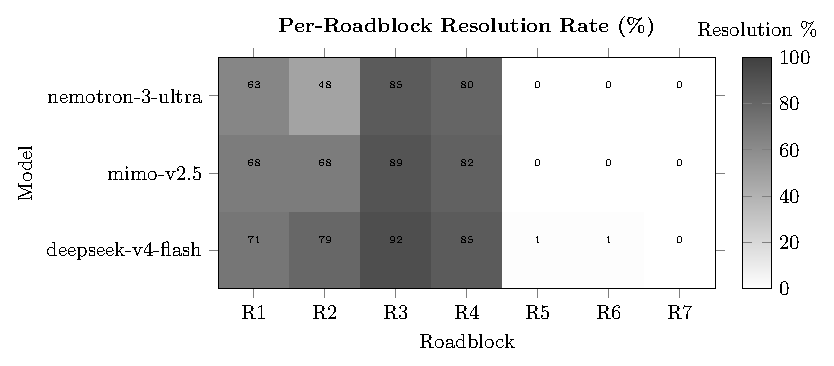
\includegraphics[width=\columnwidth]{figures/roadblock_heatmap.pdf}
\caption{Per-phase progress rates across models. R1--R4 show moderate success, but R5 (Service Rehosting) and R6 (Vulnerability Triggering) collapse to near-zero for all models.}
\label{fig:heatmap}
\end{figure}

\begin{mdframed}[linecolor=black,linewidth=1pt,backgroundcolor=gray!10,roundcorner=3pt,nobreak=true]
\noindent\textbf{Result for RQ4:} 69.8\% of all 450 runs involve simulation substitution. These outputs are often coherent and plausible, producing valid crash signals and correct exploit syntax, but they never run the real firmware binary. Real-target gating is essential to distinguish genuine reproduction from simulation.
\end{mdframed}

\subsection{Vulnerability-Class and Model Analysis (RQ5)}
% RQ5: CVE级别差异大，同架构设备成功率高
Scores range from 99.5 (CVE-2023-26315) to 23.4 (CVE-2025-34037). The top-performing CVEs involve ARM64 devices where \texttt{chroot} suffices; the bottom involve MIPS devices with encrypted firmware or unavailable downloads. Buffer overflows allow partial credit via static analysis (Phase 4); command injections require real rehosting for validation; authentication bypasses need stateful request comparisons. Vulnerability class affects the validation path but is secondary to rehosting feasibility.

\begin{mdframed}[linecolor=black,linewidth=1pt,backgroundcolor=gray!10,roundcorner=3pt,nobreak=true]
\noindent\textbf{Result for RQ5:} CVE-level scores range from 99.5 to 23.4. Success correlates strongly with target architecture: ARM64 devices allowing \texttt{chroot}-based rehosting achieve full reproduction, while MIPS devices requiring QEMU almost universally fail at R5.
\end{mdframed}

\subsection{Graded vs.\ Binary Metrics (RQ6)}
% RQ6: graded评分揭示二元评分隐藏的差异
Under binary evaluation, 143/150 pairs (95.3\%) would be failures (R6 $<$ 15/20). Graded scoring reveals a 23.5-point spread (41.7--65.2) and a stage funnel invisible to binary metrics. Best-of-three scoring adds $\sim$10 points over per-run averages, with stronger models showing larger variance (e.g., \texttt{glm-5.2}: +14.3), suggesting that succeeding at least once is itself a capability dimension.

\begin{mdframed}[linecolor=black,linewidth=1pt,backgroundcolor=gray!10,roundcorner=3pt,nobreak=true]
\noindent\textbf{Result for RQ6:} Evidence-grounded scoring reveals distinctions hidden by binary success. Binary evaluation classifies 95.3\% as failures, but graded scoring shows a 23.5-point spread. The stage funnel, simulation-substitution rate, and plan--execution gap are all invisible under binary metrics.
\end{mdframed}
